\documentclass[10pt]{article}
\usepackage[margin=1in]{geometry}
\usepackage{parskip}
\usepackage{microtype}
\usepackage{natbib}
\usepackage{graphicx}
\usepackage{amsmath}
% \usepackage{txfonts}

\graphicspath{ {figures/} }
\linespread{1.3}


\begin{document}

\title{Distinguishing NFW and Isothermal Density Profiles with Weak Gravitational Lensing}
\author{Ian Holst and Doyee Byun}
\date{\today}
\maketitle

\begin{abstract}
We examine the feasibility of distinguishing NFW and cored isothermal density profiles using weak gravitational lensing shear.

We model lenses in the two different profiles, as well as background galaxies to be lensed.
Analyzing the simulated data of these lensed galaxies gives us insight into how we can distinguish the differences between the two profiles.
This method is expected to be helpful in the analysis of real observation data in the future.
\end{abstract}


\section{Introduction}
Gravitational lensing allows us to investigate the matter density distributions of cosmic objects by observing the characteristic distortions imparted on other objects in the background. The principle is applicable on a large range of scales, from all-sky mass maps based on cosmic microwave background shear to studies of individual galaxies and clusters. In particular, by observing the coherent distortions of many background galaxies, the shear profile, and consequently the density profile of a foreground halo lens may be determined.

Two commonly used density profiles in the field are the isothermal profile and the Navarro-Frenk-White (NFW) profile. The NFW profile has been found to fit simulated dark matter halos very well \citep{}, while the isothermal profile .
Both profiles have infinite extent

Lensing offers one of the only ways to probe the distribution
In this paper, we will investigate the distinguishability of
given galaxy-galaxy lensing data

We start with introducing the general characteristics of spherical density profiles, followed by cored isothermal and NFW profiles.
We then describe the purpose of our project, to distinguish between NFW and isothermal profiles, in detail.
The goal of this project is to devise a method to analyze lensed galaxy cluster data and find which density profile is more probable between the isothermal and NFW profiles.
In order to do so, we generate simulated data sets and analyze them to find the more probable profiles they would fit into.
This analysis method is expected to be usable in determining the characteristics of real observed data as well.



Estimating ellipticity has well-documented issues [cite] due to noise and PSF


We describe the common characteristics of spherical density profiles.
Here we define our conventions for various lensing quantities, which mainly conform to those used by \citet{Dodelson2017}. We use the thin lens approximation and assume spherical lens profiles.
Consider such a spherically symmetric halo density profile $\rho(r)$

The lens halo is located at an angular diameter distance $D_L$ from the observer and we want to consider its effects on a source object behind it at an angular diameter distance $D_S$.

The projected surface density at radius R on the projected plane is defined, considering the z axis to be along the line of sight:
\begin{equation}
\Sigma(R) = \int_{-\infty}^{\infty}{dz\ \rho(\sqrt{R^2 + z^2})}
\end{equation}

An important related measure in gravitational lensing is the average projected surface density within radius R:
\begin{equation}
\overline{\Sigma}(R) = \frac{1}{\pi R^2} \int_0^{2\pi}{d\phi \int_0^{R}{dR'~\Sigma(R')R'}}
\end{equation}

The critical surface density marks the typical boundary between what is considered strong and weak lensing:
\begin{equation}
\Sigma_\mathrm{crit} = \frac{c^2}{4\pi G} \frac{D_S}{(D_S - D_L) D_L}
\end{equation}

At small angles, we can assume from small angle approximations that $R = D_L \theta$.

We also define the convergence, $\kappa$ to be
\begin{equation}
\kappa(\theta) = \frac{\Sigma(\theta)}{\Sigma_\mathrm{crit}}
\end{equation}

Strong lensing features take over when the convergence is greater than one.
Tangential shear, along with the components of shear are shown as follows.
\begin{equation}
\gamma_t(\theta) = \overline{\kappa}(\theta) - \kappa(\theta)
\end{equation}

The tangential shear is decomposed into two components, $\gamma_1$ and $\gamma_2$. $\gamma_1$ represents stretching along the $\theta_x$ and $\theta_y$ axes, and $\gamma_2$
\begin{equation}
\begin{split}
\gamma_1 = -\gamma_t \cos{2\phi}\\
\gamma_2 = -\gamma_t \sin{2\phi}
\end{split}
\end{equation}

It can be shown that for a spherical lens profile, the only component of shear $\gamma$ should be the tangential shear, $\gamma_t$:
\citep{Dodelson2017}
\begin{equation}
\gamma = \gamma_t = \sqrt{{\gamma_1}^2 + {\gamma_2}^2} = -\gamma_1 \cos{2\phi} -\gamma_2 \sin{2\phi}
\end{equation}

Deflection angle is
\begin{equation}
\vec{\alpha}(\vec{\theta}) = \overline{\kappa}(\theta)\vec{\theta}
\end{equation}
\begin{equation}
\vec{\beta} = \vec{\theta} - \vec{\alpha} = (1 - \overline{\kappa}(\theta))\vec{\theta}
\end{equation}

while ellipticity is
\begin{equation}
\epsilon_i = \frac{2 \gamma_i/(1 - \kappa)}{1 + \gamma^2/(1 - \kappa)^2}
\end{equation}
\begin{equation}
\epsilon =  -\epsilon_1 \cos{2\phi} -\epsilon_2 \sin{2\phi}
\end{equation}



\section{Cored Isothermal Sphere Profile}
The cored isothermal sphere (CIS) profile is related to the singular isothermal sphere profile, which is often used to describe halos and other collapsed astrophysical objects because of its simple formulation. Unlike the singular isothermal sphere, the cored isothermal sphere does not have a density singularity at its center due to a finite core radius $r_c$. The CIS density profile is defined:

\begin{equation}
\rho_\mathrm{iso}(r) = \frac{\sigma^2}{2\pi G (r^2 + {r_c}^2)}
\end{equation}

where $\sigma^2$ is the velocity dispersion.
https://arxiv.org/pdf/astro-ph/9810164.pdf
% \begin{equation}\Sigma_\mathrm{iso}(R) = \frac{\sigma^2}{2 G \sqrt{R^2 + {r_c}^2}}
% \end{equation}
%
% \begin{equation}\overline{\Sigma}_\mathrm{iso}(R) = \frac{\sigma^2 \left(\sqrt{R^2 + {r_c}^2} - r_c \right)}{G R^2}
% \end{equation}
%
% In terms of angles:

\begin{equation}
\Sigma_\mathrm{iso}(\theta) = \frac{\sigma^2}{2 G D_L \sqrt{\theta^2 + {\theta_c}^2}}
\end{equation}

\begin{equation}
\overline{\Sigma}_\mathrm{iso}(\theta) = \frac{\sigma^2 \left(\sqrt{\theta^2 + {\theta_c}^2} - \theta_c \right)}{G D_L \theta^2}
\end{equation}

\begin{equation}
\gamma_\mathrm{iso}(\theta) = \frac{\sigma^2 \left(\sqrt{\theta^2 + {\theta_c}^2} - \theta_c \right)}{\Sigma_\mathrm{crit} G D_L \theta^2} - \frac{\sigma^2}{2 \Sigma_\mathrm{crit} G D_L \sqrt{\theta^2 + {\theta_c}^2}}
\end{equation}

We switch dependence from $\sigma^2$ to $M_{200}$ with:

\begin{equation}
\sigma^2 = \frac{M_{200} G}{2 \left( r_{200} - r_c \arctan{\left(\frac{r_{200}}{r_c}\right)} \right)}
\end{equation}

This is derived from the definition of $M_{200}$:

\begin{equation}
M_{200} = 200 \rho_\mathrm{crit} \frac{4}{3} \pi {r_{200}}^3
\end{equation}
\begin{equation}
M_{200} = M_\mathrm{enc}(r_{200}) = \frac{2 \sigma^2}{G} \left( r_{200} - r_c \arctan{\left(\frac{r_{200}}{r_c}\right)} \right)
\end{equation}
\begin{equation}
r_{200} = \left( \frac{3 M_{200}}{800 \pi \rho_\mathrm{crit}} \right)^{1/3}
\end{equation}

The ellipticity equations, while not quite elegant, are trivial to calculate from the shear.

\begin{figure}
    \centering
    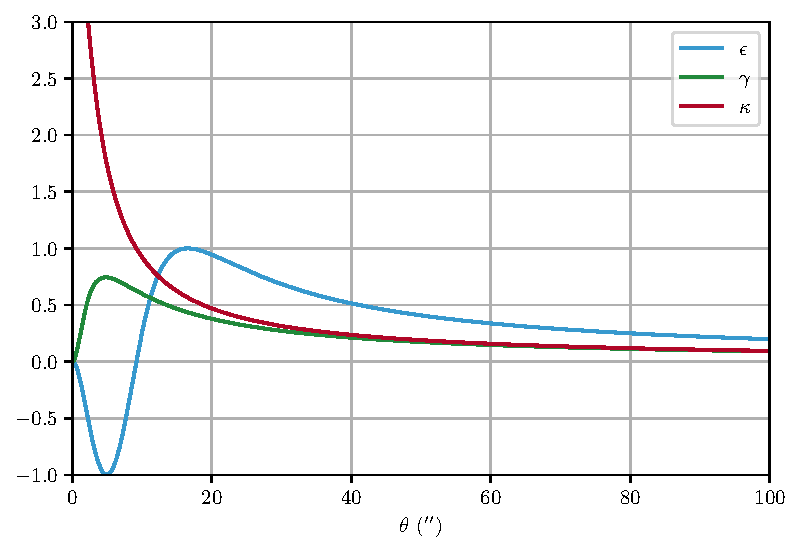
\includegraphics[width=0.8\textwidth]{isothermalproperties.pdf}
    \caption{Lensing quantities for a CIS profile with $M_{200} = 10^{15} M_\odot$ and $r_c = 10$ kpc.}
    \label{}
\end{figure}


\section{Navarro-Frenk-White (NFW) Profile}

\begin{equation}
\rho_\mathrm{NFW}(r) = \frac{\rho_\mathrm{crit} \delta_c}{(r/r_s)\left(1 + r/r_s\right)^2}
\end{equation}

What redshift is $\rho_\mathrm{crit}$ evaluated at? - at halo redshift - can we use current time?

% \begin{equation}\Sigma_\mathrm{NFW}(R) = \frac{2 \rho_\mathrm{crit} \delta_c r_s}{(R/r_s)^2 - 1} \left(1 - \frac{2}{\sqrt{(R/r_s)^2 - 1}}  \arctan\left(\sqrt{\frac{R/r_s - 1}{R/r_s + 1}} \right) \right)
% \end{equation}
%
%
% \begin{equation}\overline{\Sigma}_\mathrm{NFW}(R) = \frac{4 \rho_\mathrm{crit} \delta_c r_s}{(R/r_s)^2} \left(
%     \frac{2}{\sqrt{(R/r_s)^2 - 1}} ~\arctan\left(\sqrt{\frac{R/r_s - 1}{R/r_s + 1}} \right) + \ln{\left(\frac{R/r_s}{2}\right)}
% \right)
% \end{equation}
%
% In terms of angles:

\begin{equation}
\Sigma_\mathrm{NFW}(\theta) = \frac{2 \rho_\mathrm{crit} \delta_c D_L \theta_s}{(\theta/\theta_s)^2 - 1} \left(1 - \frac{2}{\sqrt{(\theta/\theta_s)^2 - 1}} \arctan\left(\sqrt{\frac{\theta/\theta_s - 1}{\theta/\theta_s + 1}} \right) \right)
\end{equation}

\begin{equation}
\overline{\Sigma}_\mathrm{NFW}(\theta) = \frac{4 \rho_\mathrm{crit} \delta_c D_L \theta_s}{(\theta/\theta_s)^2} \left(
    \frac{2}{\sqrt{(\theta/\theta_s)^2 - 1}} ~\arctan\left(\sqrt{\frac{\theta/\theta_s - 1}{\theta/\theta_s + 1}} \right) + \ln{\left(\frac{\theta/\theta_s}{2}\right)}
\right)
\end{equation}

Similar convention used by \citet{Bartelmann2001}

\begin{equation}
\gamma_\mathrm{NFW}(\theta) = \frac{\overline{\Sigma}_\mathrm{NFW}(\theta) - \Sigma_\mathrm{NFW}(\theta)}{\Sigma_\mathrm{crit}}
\end{equation}

Can calculate ellipticities from tangential shear.

We switch the dependence to $M_{200}$ and $c$ with:

\begin{equation}
\delta_c = \frac{200}{3} \frac{c^3}{\ln(1 + c) - c/(1 + c)}
\end{equation}
\begin{equation}
r_s = \frac{r_{200}}{c}
\end{equation}
\begin{equation}
r_{200} = \left( \frac{3 M_{200}}{800 \pi \rho_\mathrm{crit}} \right)^{1/3}
\end{equation}
\begin{equation}
c = \frac{r_{200}}{r_s}
\end{equation}

\begin{figure}
    \centering
    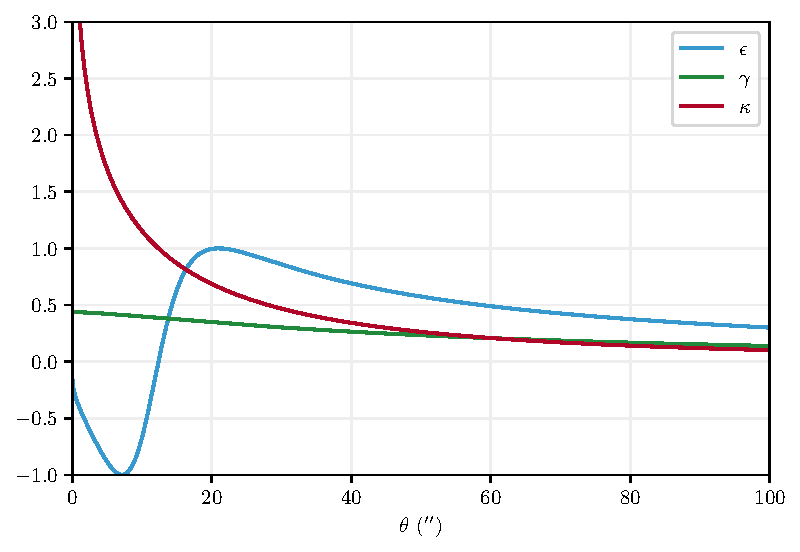
\includegraphics[width=0.8\textwidth]{nfwproperties.pdf}
    \caption{Lensing quantities for a NFW profile with $M_{200} = 10^{15} M_\odot$ and $c = 10$.}
    \label{}
\end{figure}




\section{Methods}

\subsection{Modelling of Foreground Lens and Background Galaxies}
Based on the calculations shown above, we have modelled singular lenses corresponding to each density profile.
 Background galaxies have been generated via randomization of angular coordinates.

\begin{enumerate}
    \item Consider single foreground lens halo with many background galaxies.
    \begin{itemize}
        \item Start with one NFW halo, then maybe consider more tests.
    \end{itemize}
    \item Construct background galaxies:
    \begin{itemize}
        \item Number density on sky: 50 galaxies/square arcminute (LSST, https://arxiv.org/pdf/1305.0793.pdf)
        \item Intrinsic ellipticity drawn from Gaussian distribution with $\mu=0, \sigma=0.2$ (consistent with https://arxiv.org/pdf/1509.05058.pdf)
        \item Assume they are all that the same distance $D_S$ since this can be determined by redshift (neglecting some noise)
    \end{itemize}
    \item Recommended values:
    \begin{itemize}
        \item $z_L = 0.3$ (bullet cluster)
        \item $z_S = 1.0$ (Hubble Deep Field) (also consistent with https://arxiv.org/pdf/1509.05058.pdf)
        we use the planck 2015 results
        \item $M_{halo} = 10^{15} M_\odot$
    \end{itemize}
\end{enumerate}

\subsection{Generating Simulated Data}
We applied the shear and deflection angles to background galaxies to get simulated data: $N$ sets of $\epsilon_1$, $\epsilon_2$, $\theta_1$, $\theta_2$

\begin{figure}
    \centering
    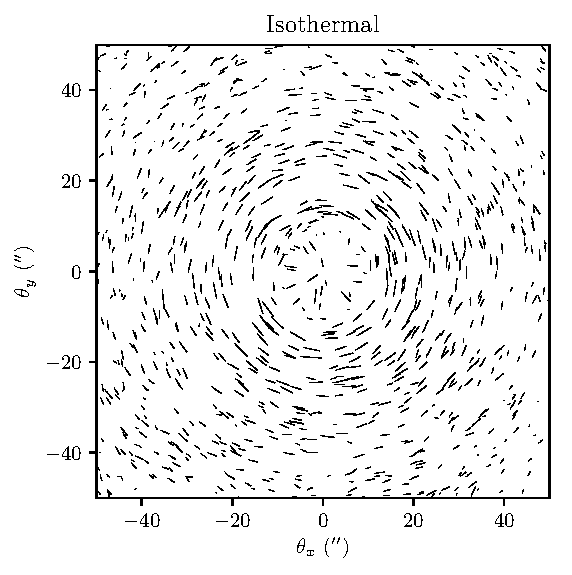
\includegraphics[width=0.49\textwidth]{isothermalellipticities.pdf}
    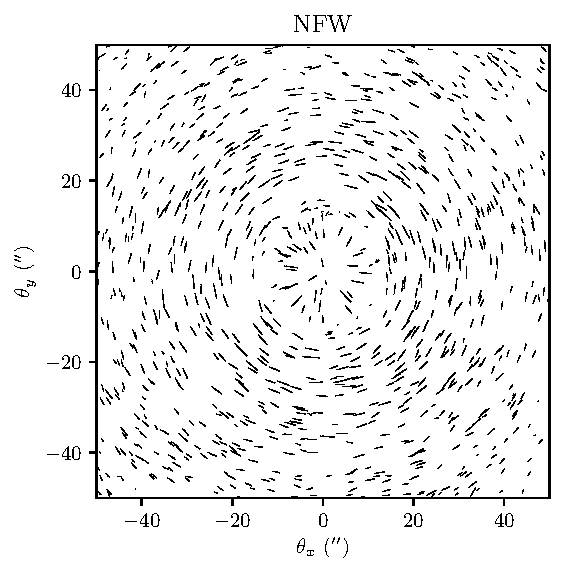
\includegraphics[width=0.49\textwidth]{nfwellipticities.pdf}
    \caption{plots}
    \label{}
\end{figure}


\subsection{Data Analysis and Density Profile Determination}
\begin{enumerate}
\item Bin galaxies in annuli by $\theta$ value (use log bins for theta)
\item Calculate mean and standard deviation of ellipticity
\item Attempt to fit both NFW and isothermal profiles, see if the fit is distinguishable
\end{enumerate}

What theta range should we look at? (5 arcminutes?)

How to properly do sigma contours?

\section{Results}

\begin{figure}
    \centering
    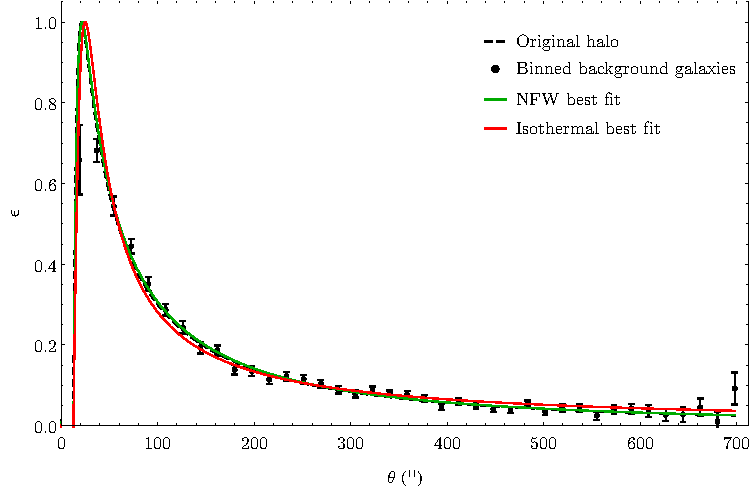
\includegraphics[width=0.9\textwidth]{comparison.pdf}
    \caption{plots}
    \label{}
\end{figure}

\section{Conclusions}

Like (COMPARISONS BETWEEN ISOTHERMAL AND NFW MASS PROFILES
FOR STRONG-LENSING GALAXY CLUSTERS), we find that the strong lensing regime provides the most
But also, weak lensing can in fact provide sufficient distinguishability

has been applied to observations before
https://arxiv.org/pdf/astro-ph/9602053.pdf
but not in the context of comparing density profiles using for strong and weak
but this is highly dependent on good data

http://iopscience.iop.org/article/10.1086/590049/pdf looked at NFW vs isothermal in strong lensing with a focus on arcs, and found differing levels of distinguishibility for different lenses.

https://arxiv.org/pdf/1101.0650.pdf - our results don't match

From our data analysis, we were able to find the more probable density profile of a simulated data set.
Since the simulated data is based on the NFW and isothermal profile models, we were able to decisively distinguish between the two.
When analyzing real observed data, we expect the probability ratios to be relatively more even.
Future goals include the use of these methods to analyze observed data of galaxy clusters to find the density profile of their lenses.

Where to go from here?


\bibliographystyle{plainnat}
\bibliography{references}

\end{document}
